% TM - Theorical
%%%%%%%%%%%%%%%%%%%%%%%%%%%%%%%%%%%%%%%%%%%%%

%%%%%%%%%%%%%%%%%%%%%%%%%%%%%%%%%%%%%%%%%%%%%%%%%%%%%%%%%%%%%%%%%%%%%%%%%
% EN
%\section{Transportation model}

% FR
\section{Modèle de Transport}

% EN
%A transportation modelling is method for determining a traffic on road in focused area. Our goal is determine number of trip per road in road network from socio-economic and demographic data.

%Traditional transportation modelling have a several independent step (e.g trip generation, trip destination, ...). Our implementation of transportation modelling consist from 3 steps.

% FR
Un modèle de transport est une méthode déterminant un traffic sur les routes ciblé sur une zone décidée. Notre objectif est de déterminer un élément quantitatif d'afflux par route sur un réseau routier à partir de données socio-économiques et démographiques.

La modélisation de transport traditionnels possède plusieurs étape indépendantes (par exemple la génération de voyage, voyage destination, ...). Notre mise en oeuvre de la modélisation du transport se composent de 3 étapes :

% EN
% \begin{itemize}
%   \item[ ] \textbf{trip generation} - I this part we want to determine number of trip origin, destination in zones. This step is depend on data (e.g demographic data, socio-economic data, weather, local habits, ...). Quality of model depend a lot on these data.
%   \item[ ] \textbf{trip destination} - In this section we want determine \textit{transportation matrix} $T$ (OD matrix). It say how many people travel from zone $i$ to zone $j$. For it was used Gravity model.
%   \item[ ] \textbf{counting traffic} - This is last step.  We compute traffic for every road link (edge of graph).
% \end{itemize}

% FR
\begin{itemize}
  \item[ ] \textbf{la génération des déplacements} - Dans cette partie, nous voulons déterminer le nombre d'origine du voyage, la destination dans les zones. Cette étape est dépendent de données (par exemple des données démographiques, des données socio-économiques, météorologiques, les habitudes locales, ...). La qualité du modèle dépendra beaucoup de ces données.

  \item[ ] \textbf{la destination des déplacements} - Dans cette section nous voulons déterminer \textit{transportation matrix} $T$ (OD matrix). Cette matrice permet de dénombrer les  voyages entre une zone $i$ vers une zone $j$. Pour ce faire, nous utiliserons un modèle de gravité (Gravity Model).


  \item[ ] \textbf{Dénombrement du traffic} - Cette étape est la dernière. Nous calculons le trafic pour chaque liaison routière (bord du graphique).
\end{itemize}

% EN
%In upcoming section following expressions will be used:

% \begin{tabular}{ll}
%   $T$ & transportation matrix (number of trips between zones)\\
%   $C$ & travel cost matrix (between zones) \\
%   $T_i, T_j$ & sum value in row/column in $T$\\
%   $n$ & number of zones (size of matrix)
% \end{tabular}

% FR
Dans la suite de ce chapitre, les expressions suivantes vont être utilisées :

\begin{tabular}{ll}
  $T$ & transportation matrix (nombre de voyage entre deux zones)\\
  $C$ & travel cost matrix (le coup du voyage entre deux zones) \\
  $T_i, T_j$ & somme des valeurs en ligne/colonne dans $T$\\
  $n$ & nombre de zone (taille de la matrice)
\end{tabular}


%%%%%%%%%%%%%%%%%%%%%%%%%%%%%%%%%%%%%%%%%%%%%%%%%%%%%%%%%%%%%%%%%%%%%%%%%

% EN
%\subsection{Trip destination}

% FR
\subsection{Destinations des déplacements}

% EN
% For determine transportation matrix $T$ was used Gravity model:
% $$T_{ij} = K_i K_j T_i T_j f(C_{ij})$$
% where
% $$T_i = \sum_{j = 1}^{n} T_{ij}$$
% $$T_j = \sum_{i = 1}^{n} T_{ij}$$
% $$K_i = \frac{1}{\sum_{j} K_j T_j f(C_{ij})}$$
% $$K_j = \frac{1}{\sum_{i} K_i T_i f(C_{ij})}$$
% where in our case $$f(x) = x^{-2}$$
% $T_i$ is number of trips outcoming from the zone (origin in the zone) $i$, $T_j$ is number of trips incoming to the zone (destination in zone) $j$. So sometimes transportation matrix is called \textit{OD Matrix}. 

% FR
Pour déterminer la matrice de transport $T$ nous avons utilisé la méthode Gravity Model :
$$T_{ij} = K_i K_j T_i T_j f(C_{ij})$$
où
$$T_i = \sum_{j = 1}^{n} T_{ij}$$
$$T_j = \sum_{i = 1}^{n} T_{ij}$$
$$K_i = \frac{1}{\sum_{j} K_j T_j f(C_{ij})}$$
$$K_j = \frac{1}{\sum_{i} K_i T_i f(C_{ij})}$$
où dans notre cas $$f(x) = x^{-2}$$
$T_i$ est le nombre de voyage sortant de la zone (origine dans la zone) $i$, $T_j$ est le nombre de voyage entrant dans la zone (destination dans la zone) $j$. Quelques fois, la matrice de transpor est appellée \textit{OD Matrix} (Origine - Destination).


% EN
% Now we must determine $K_i$ and $K_j$. We used iterative proportional fitting. It is iterative solution. First we compute $T^1$ with $K_i, K_j = 1$. After we can use iteration equation for $T$:
% $$T_{ij}^{p} = \frac{Z_i}{T_i^{m-1}} T_{ij}^{k-1}$$
% $$T_{ij}^{k} = \frac{Z_j}{T_j^{m-1}} T_{ij}^{p}$$
% where $Z_i$ and $Z_j$ are origin and destination trips (we know), $k$ is iteration.

% FR
Maintenant nous devons déterminer $K_i$ et $K_j$. Pour ce faire nous avons utilisé un ajustement proportionnel itératif. Premièrement nous calculons $T^1$ avec $K_i, K_j = 1$. Ensuite nous pouvons utiliser une équation itérative pour $T$:
$$T_{ij}^{p} = \frac{Z_i}{T_i^{m-1}} T_{ij}^{k-1}$$
$$T_{ij}^{k} = \frac{Z_j}{T_j^{m-1}} T_{ij}^{p}$$
où $Z_i$ et $Z_j$ sont les voyages d'origine et de destination, $k$ est une itération.

Exemple:
$$Z = (\begin{array}{ccc}
24  & 34  & 15\\
\end{array})$$
$$
C = \left(\begin{array}{ccc}
0& 10 &20 \\
10& 0 &15 \\
20 & 15& 0 \\
\end{array}\right) \Rightarrow T^0 = \left(\begin{array}{ccc}
       0  & 8.16000  &  0.90000\\
   8.16000  &     0  & 2.26667\\
   0.90000  & 2.26667  &    0\\
\end{array}\right) \Rightarrow$$
$$T^0 = \left(\begin{array}{ccc}
       0  & 8.16000  &  0.90000\\
   8.16000  &     0  & 2.26667\\
   0.90000  & 2.26667  &    0\\
\end{array}\right) \Rightarrow T^1 = \left( \begin{array}{ccc}
    0.00000 &  22.71648 &   3.65832 \\
   20.68579 &   0.00000 &  11.34168 \\
    3.31421 &  11.28352 &   0.00000 \\
\end{array} \right)$$
Après une itération, les coefficients sont:
$$\frac{Z_i}{\sum_j T_{ij}} = \left(\begin{array}{c}
0.90996 \\
1.06159  \\
1.02756\\
\end{array}\right) \quad \frac{Z_j}{\sum_i T_{ij}} = \left(\begin{array}{ccc}
0  & 0 & 0\\
\end{array}\right)$$

%%%%%%%%%%%%%%%%%%%%%%%%%%%%%%%%%%%%%%%%%%%%%%%%%%%%%%%%%%%%%%%%%%%%%%%%%

% EN
% \subsection{Count traffic}

% FR
\subsection{Dénombrement du traffic}

% EN
% Now we know how many people travel from zone $i$ to zone $j$, so we can find path from $i$ to $j$ and 
% record this value into every edges in path. So we have to compute $z^2$ shortest paths ($z$ is number of zones). Because we have to compute shortest path between all pair of zones.

% FR
Maintenant, nous savons combien de personnes voyagent de la zone $i$ à la zone $j$, afin que nous puissions trouver le chemin le plus court de $i$ à $j$ et enregistrer cette valeur dans tous bords de la matrice nous devons calculer $z^2$, où $z$ est le nombre de zones. Nous devons donc calculer plus court chemin entre les deux zones OD.

% EN
%In our solution we compute N paths for every pair of zones (finally will be compute $N z^2$ paths). Every path is based on another cost. Cost is based on length, time and vertical distance. Final cost is linear combination these partition cost.

% FR
Dans notre solution, nous calculons N chemins pour toutes les paires OD (finallement, nous calculons $N z^2$ chemins). Chaque chemin est basé sur un autre coût. Le coût est basé sur la longueur, le temps et la destination verticale. Le coût final est combinaison linéaire de ces coûts de partition.

$$c = \left(\begin{array}{ccc}
k_t & k_l & k_h\\
\end{array}\right) \left( \begin{array}{c}
t\\
l\\
h\\
\end{array} \right)$$

% EN
% where $c$ is cost, $t$ is time, $l$ is length and $h$ is vertical distance. Number of trip (traffic between two zones) is splitted between those paths. In Fig. \ref{img.paths} you can see multipath (same pareto optimal paths) between two zones.

% FR
où $c$ est le coût, $t$ le temps, $l$ la longueur et $h$ la distance verticale. Nombre de voyage (traffic entre deux zones) est découpée entre ces parties. Sur la figure \ref{img.paths} on peut voir les multi-chemins (même chemins optimaux) entre deux zones.

\begin{figure}
  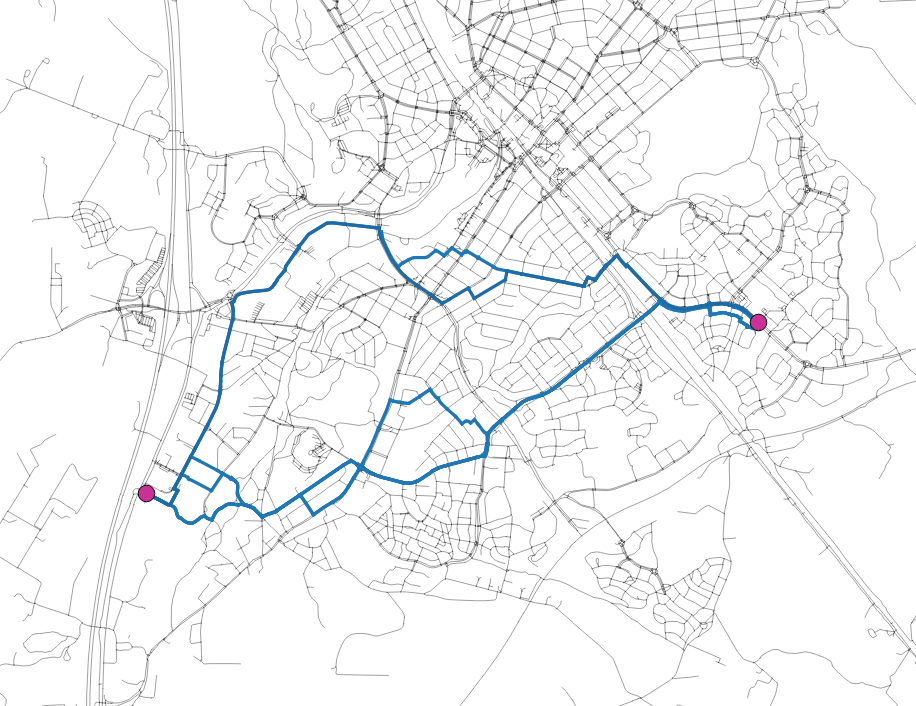
\includegraphics[width=12cm]{img/c01-transp-model/paths.png}
  \label{img.paths}
  \caption{Possible paths between one pair of zone (multipath)}
\end{figure}